
\documentclass{ffhsthesis}

\usepackage[english,ngerman]{babel}
\usepackage[utf8]{inputenc}
\usepackage[T1]{fontenc}
\usepackage{setspace}
\usepackage{helvet}
\usepackage{graphicx}
\usepackage[table,xcdraw]{xcolor}
\usepackage{makeidx}
\usepackage[acronym]{glossaries}
\usepackage{float}
\usepackage{dirtytalk}
\usepackage{bera}
\usepackage{listings}
\usepackage{xcolor}
\usepackage{lmodern}
\usepackage{ulem}
\usepackage{hyperref}
\usepackage{natbib}
\usepackage{subfiles}
\usepackage{color}
\usepackage{booktabs}
\usepackage{environ}
\usepackage[tikz]{bclogo}
\usepackage{tikz}
\usepackage{pdfpages}

\newcommand\tab[1][1cm]{\hspace*{#1}}
\renewcommand{\familydefault}{\sfdefault}


\colorlet{punct}{red!60!black}
\definecolor{background}{HTML}{FFFFFF}
\definecolor{delim}{RGB}{20,105,176}
\colorlet{numb}{magenta!60!black}

\lstdefinelanguage{json}{
    basicstyle=\footnotesize\ttfamily,
    numbers=left,
    numberstyle=\tiny,
    stepnumber=1,
    numbersep=8pt,
    showstringspaces=false,
    breaklines=true,
    frame=lines,
    backgroundcolor=\color{background},
    literate=
     *{0}{{{\color{numb}0}}}{1}
      {1}{{{\color{numb}1}}}{1}
      {2}{{{\color{numb}2}}}{1}
      {3}{{{\color{numb}3}}}{1}
      {4}{{{\color{numb}4}}}{1}
      {5}{{{\color{numb}5}}}{1}
      {6}{{{\color{numb}6}}}{1}
      {7}{{{\color{numb}7}}}{1}
      {8}{{{\color{numb}8}}}{1}
      {9}{{{\color{numb}9}}}{1}
      {:}{{{\color{punct}{:}}}}{1}
      {,}{{{\color{punct}{,}}}}{1}
      {\{}{{{\color{delim}{\{}}}}{1}
      {\}}{{{\color{delim}{\}}}}}{1}
      {[}{{{\color{delim}{[}}}}{1}
      {]}{{{\color{delim}{]}}}}{1},
}

\definecolor{gray}{rgb}{0.5,0.5,0.5}
\definecolor{mauve}{rgb}{0.58,0,0.82}

\lstset{
    frame=tb,
    language=bash,
    aboveskip=3mm,
    belowskip=3mm,
    showstringspaces=false,
    columns=flexible,
    basicstyle=\footnotesize\ttfamily,
    numbers=left,
    numberstyle=\tiny\color{gray},
    commentstyle=\color{red},
    keywordstyle=\color{blue},
    stringstyle=\color{mauve},
    breaklines=true,
    breakatwhitespace=true,
    tabsize=3,
    numberstyle=\tiny,
    stepnumber=1,
    numbersep=8pt,
}

\usetikzlibrary{calc}
% Glossar laden
\loadglsentries{acronyms} 
\makeglossaries

\NewEnviron{workMark}[1]
  {\par\medskip\noindent
  \begin{tikzpicture}
    \node[inner sep=0pt] (box) {\parbox[t]{.99\textwidth}{%
      \begin{minipage}{.3\textwidth}
      \centering\tikz[scale=5]\node[scale=3,rotate=0]{\bcoutil};
      \end{minipage}%
      \begin{minipage}{.65\textwidth}
      \textbf{#1}\par\smallskip
      \BODY
      \end{minipage}\hfill}%
    };
    \draw[blue!75!black,line width=3pt] 
      ( $ (box.north east) + (-5pt,3pt) $ ) -- ( $ (box.north east) + (0,3pt) $ ) -- ( $ (box.south east) + (0,-3pt) $ ) -- + (-5pt,0);
    \draw[blue!75!black,line width=3pt] 
      ( $ (box.north west) + (5pt,3pt) $ ) -- ( $ (box.north west) + (0,3pt) $ ) -- ( $ (box.south west) + (0,-3pt) $ ) -- + (5pt,0);
  \end{tikzpicture}\par\medskip%
}
\NewEnviron{warningMark}[1]
  {\par\medskip\noindent
  \begin{tikzpicture}
    \node[inner sep=0pt] (box) {\parbox[t]{.99\textwidth}{%
      \begin{minipage}{.3\textwidth}
      \centering\tikz[scale=5]\node[scale=3,rotate=0]{\bcattention};
      \end{minipage}%
      \begin{minipage}{.65\textwidth}
      \textbf{#1}\par\smallskip
      \BODY
      \end{minipage}\hfill}%
    };
    \draw[red!75!black,line width=3pt] 
      ( $ (box.north east) + (-5pt,3pt) $ ) -- ( $ (box.north east) + (0,3pt) $ ) -- ( $ (box.south east) + (0,-3pt) $ ) -- + (-5pt,0);
    \draw[red!75!black,line width=3pt] 
      ( $ (box.north west) + (5pt,3pt) $ ) -- ( $ (box.north west) + (0,3pt) $ ) -- ( $ (box.south west) + (0,-3pt) $ ) -- + (5pt,0);
  \end{tikzpicture}\par\medskip%
}
\NewEnviron{reference}[1]
  {\par\medskip\noindent
  \begin{tikzpicture}
    \node[inner sep=0pt] (box) {\parbox[t]{.99\textwidth}{%
      \begin{minipage}{.3\textwidth}
      \centering\tikz[scale=5]\node[scale=2,rotate=0]{\bctrombone};
      \end{minipage}%
      \begin{minipage}{.65\textwidth}
      \textbf{#1}\par\smallskip
      \BODY
      \end{minipage}\hfill}%
    };
    \draw[green!75!black,line width=3pt] 
      ( $ (box.north east) + (-5pt,3pt) $ ) -- ( $ (box.north east) + (0,3pt) $ ) -- ( $ (box.south east) + (0,-3pt) $ ) -- + (-5pt,0);
    \draw[green!75!black,line width=3pt] 
      ( $ (box.north west) + (5pt,3pt) $ ) -- ( $ (box.north west) + (0,3pt) $ ) -- ( $ (box.south west) + (0,-3pt) $ ) -- + (5pt,0);
  \end{tikzpicture}\par\medskip%
}



%%%%%Dokument beginnt hier: %%%%%
\begin{document}

\pagenumbering{gobble}

\dokumentTyp{Bachelor-Thesis}
\studiengang{INF}
\title{Performance-Evaluation von Open Source Reporting Engines}
\subtitle{} % optional
\author{Denis E. Bittante Fanacon}
\wohnort{St. Gallen}
%\referent{Name des Referenten\\ Titel\\Unterrichtetes Fach}
\referent{Heinrich Zimmermann \\ Prof. Dr. \\ Fachbereich Enterprise Computing }
\eingereichtBei{ Dr. Oliver Kamin \\
Departement Informatik\\
Departementsleiter } 

\dedication{}


% Setzt das Zitatsquelle in eckigen Klammern [1] und nicht (1)
\setcitestyle{square}



%% Titelblatt 
\maketitle

\setcounter{page}{0}


\pagestyle{headings}    % wieder auf normale Seitenrahmen zurück schalten

\pagenumbering{Roman}  
%% Abstract Zusammenfassung und Ergebnis darzustellen
\subfile{0_abstract}





\tableofcontents	% Inhaltsverzeichnis erstellen
%\listoftables		% Tabellenverzeichnis erstellen
\cleardoublepage	% min. eine Freiseite
 
%% Für den Hauptteil normale Seitenzahlen
\pagenumbering{arabic}  % Nummerierungstyp roman | arabic




% INCLUDES der anderen Files 


\newpage
\startThesis
\pagenumbering{arabic}


\setcounter{page}{1} % Set the page counter to 1

%%%%%%%%%%%%%%%%%%%%%%%%%%%%%%%%%%%%%%%%%%%%%%%%%%%%%%%%%%%%%%%%%%%%%%%%%%%%%%%%%%%%%%%%%%%%
%%%%%%%%%%%%%%%%%%%%%%%%%%%%             CHAPTERS          %%%%%%%%%%%%%%%%%%%%%%%%%%%%%%%%%
%%%%%%%%%%%%%%%%%%%%%%%%%%%%%%%%%%%%%%%%%%%%%%%%%%%%%%%%%%%%%%%%%%%%%%%%%%%%%%%%%%%%%%%%%%%%

\subfile{mainpart/1_einleitung}

\subfile{mainpart/2_grundlagen}

\subfile{mainpart/3_methodik_prototyp}

\subfile{mainpart/3_methodik_evaluation}

\subfile{mainpart/4_analyse}

\subfile{end/erfahrungsbericht}

%%%%%%%%%%%%%%%%%%%%%%%%%%%%%%%%%%%%%%%%%%%%%%%%%%%%%%%%%%%%%%%%%%%%%%%%%%%%%%%%%%%%%%%%%%%%
%%%%%%%%%%%%%%%%%%%%%%%%%%%%       ENDE  CHAPTERS          %%%%%%%%%%%%%%%%%%%%%%%%%%%%%%%%%
%%%%%%%%%%%%%%%%%%%%%%%%%%%%%%%%%%%%%%%%%%%%%%%%%%%%%%%%%%%%%%%%%%%%%%%%%%%%%%%%%%%%%%%%%%%%


% Glossar ausgeben
\clearpage
\printglossary
\clearpage

\printglossary[type=\acronymtype]


\listoffigures

% Bibliography 

\bibliographystyle{IEEEtran}
\bibliography{references.bib}

\newpage

%Selbständigkeitserklärung
\subfile{anhang/erklaerung}
\clearpage
% Anhang falls es keinen Anhang hat dann löschen
\chapter*{Anhang}

\iffalse
Nr. Kriterien Gewichtung\newline
1 Erfassung des Themas 10/100 \newline
1.1. Definition des Themas, Problemstellung\newline
1.2. Problemabgrenzung\newline
1.3. Zielsetzung\newline
1.4 Anwendungsorientierung\newline

2 Theoretische Fundierung 20/100\newline
2.1. Relevante theoretische Ansätze\newline
2.2. Literatur\newline

3 Methodik 30/100\newline
3.1. Auswahl der Methodik und deren Begründung\newline
3.2. Korrektheit der Methodenanwendung\newline
3.3. Vollständigkeit der Methodik in Bezug zur Zielsetzung\newline

4 Resultate/Erkenntnisgewinn 27.5/100\newline
4.1. Nachvollziehbarkeit\newline
4.2. Nutzen der Arbeit für die Praxis\newline
4.3 Bewertung der Ergebnisse\newline
4.4. Originalität\newline

5 Formales und Stilistisches 7.5/100\newline
5.1. Strukturierung\newline
5.2. Formatierung/Layout\newline
5.3 Rechtschreibung, Ausdruck, Stil\newline
5.4 Zitierweise, Literaturhinweise\newline

6 Poster /100\newline
6.1. Erfüllung des AIDA-Prinzips, gemäss Ratgeber\newline
6.2. Inhalt, Aussage, Verständlichkeit\newline
6.3 Visuelle Grammatik, gemäss Ratgeber\newline
\fi


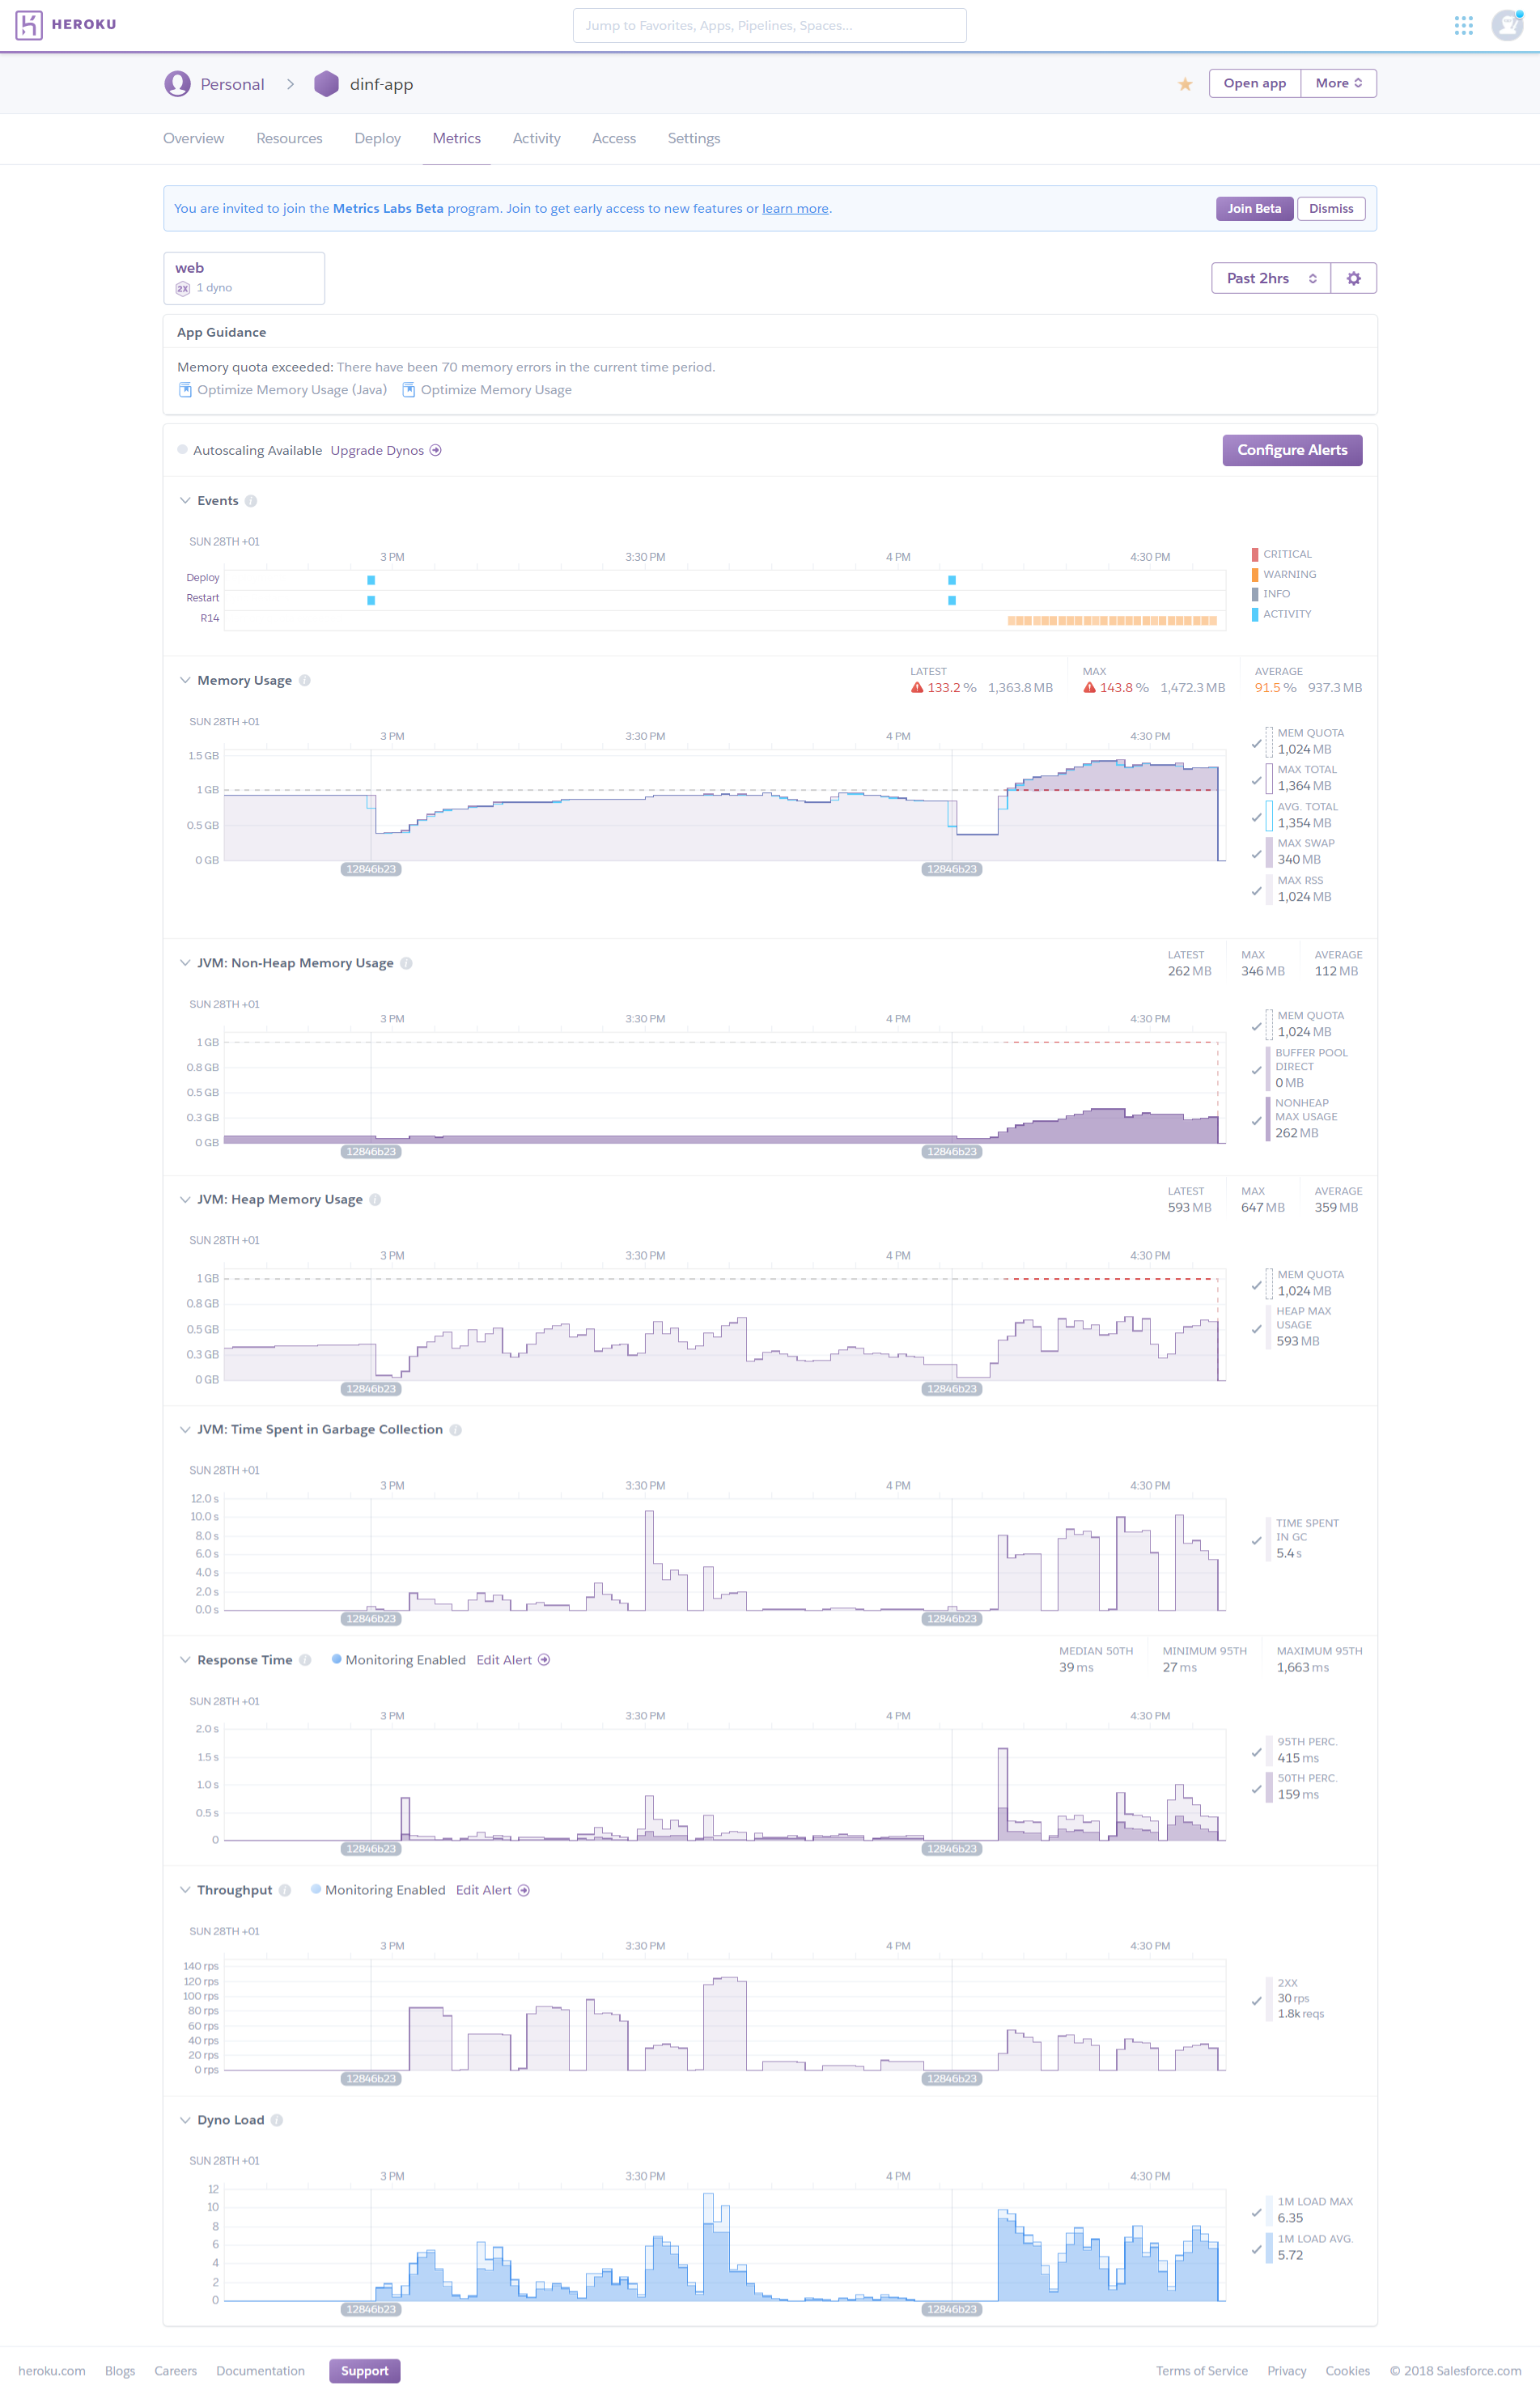
\includegraphics[width=350pt ]{anhang/screencapture-dashboard-heroku-apps-dinf-app-metrics-web-1517153971214.png}\newline

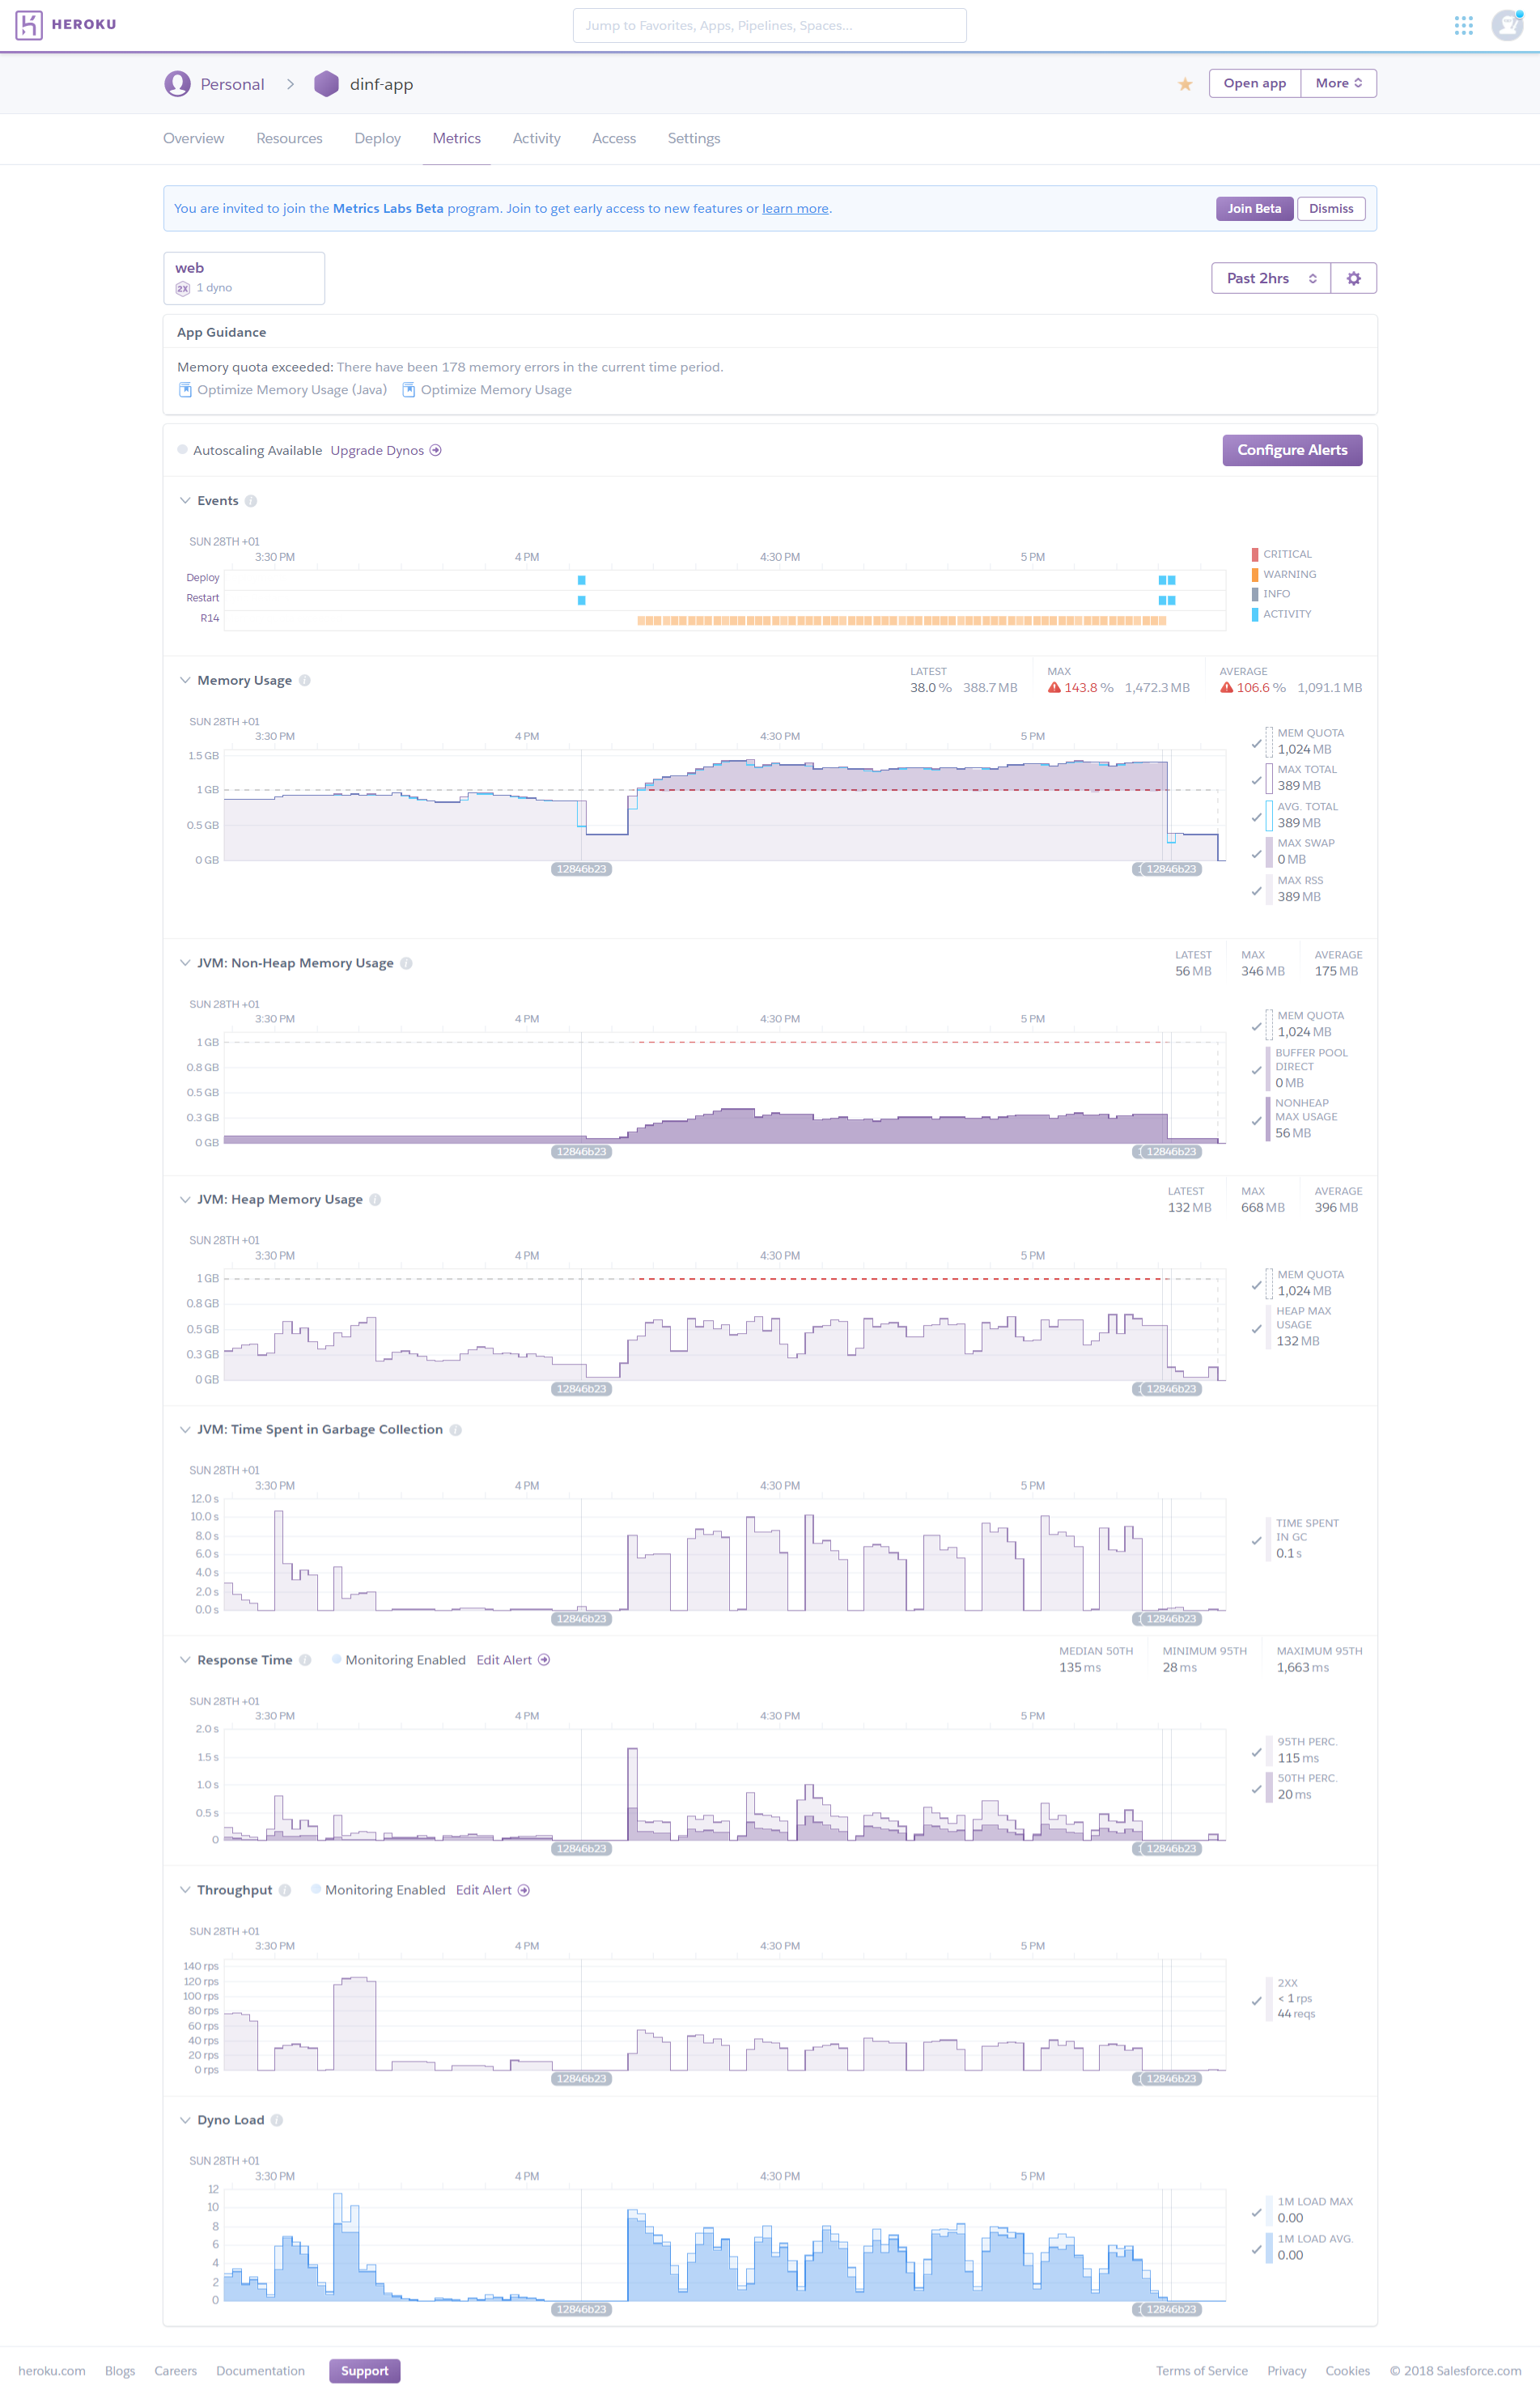
\includegraphics[width=350pt ]{anhang/screencapture-dashboard-heroku-apps-dinf-app-metrics-web-1517156607741.png}\newline


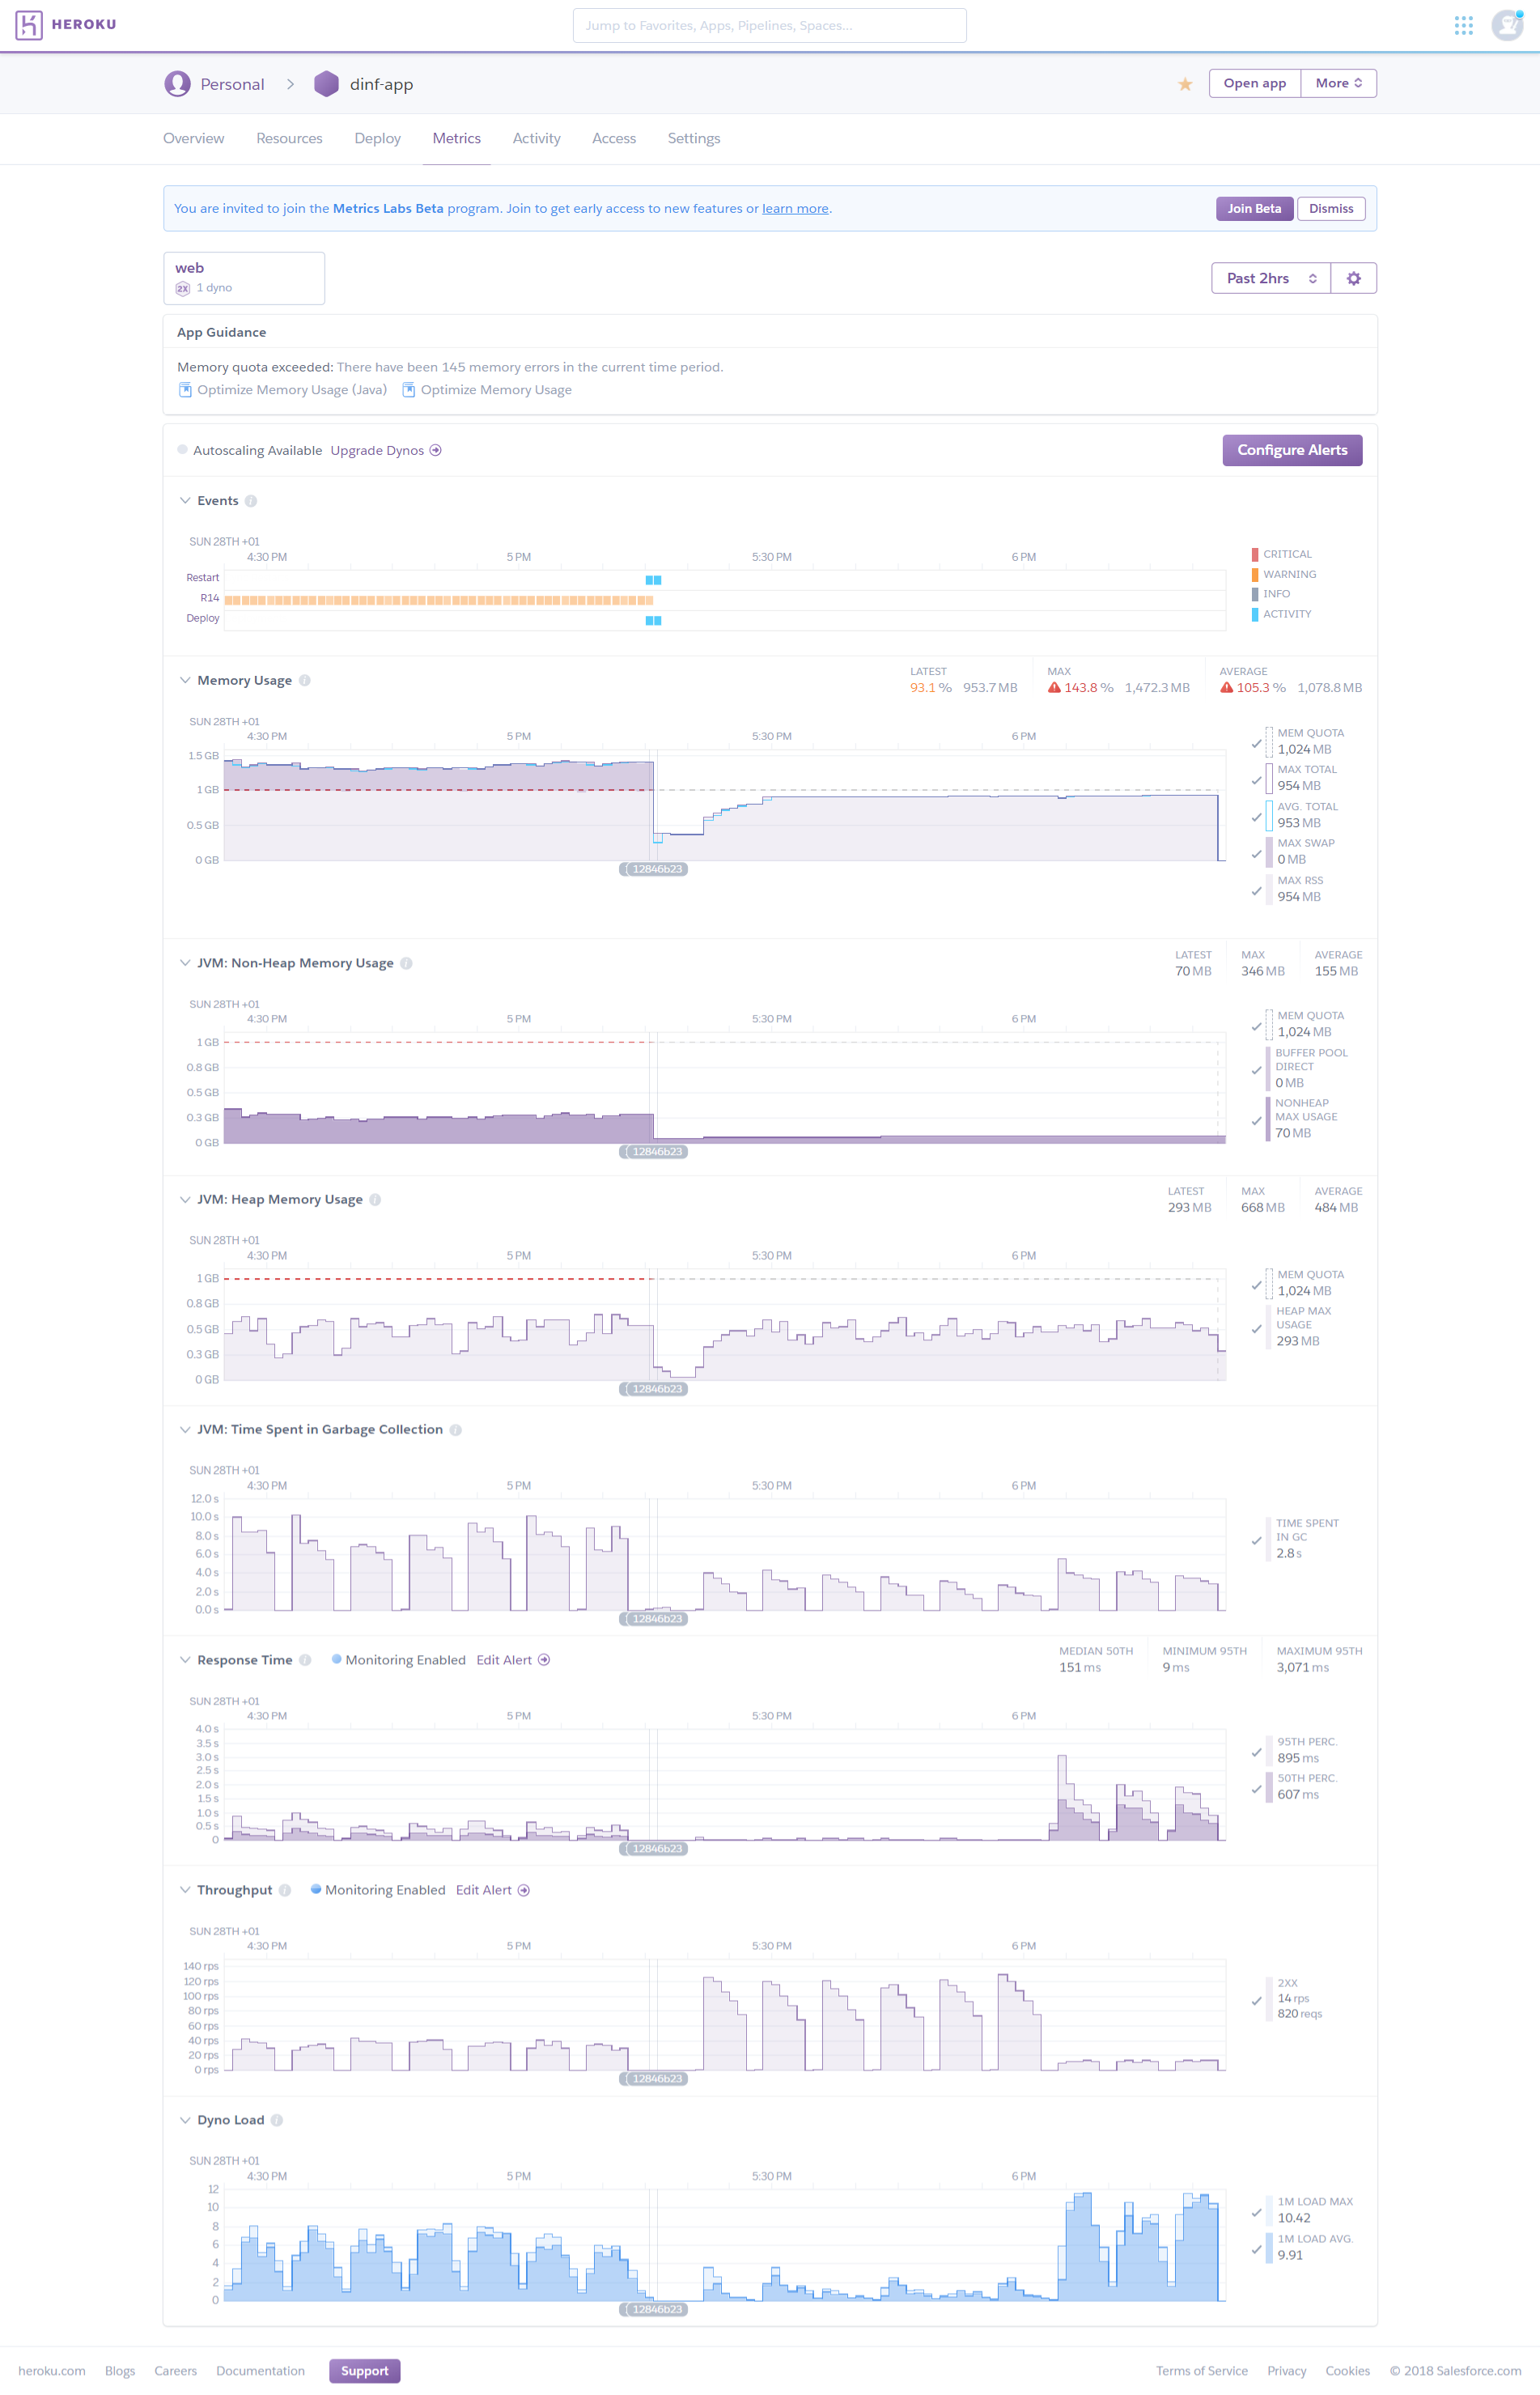
\includegraphics[width=350pt]{anhang/screencapture-dashboard-heroku-apps-dinf-app-metrics-web-1517160269318.png}\newline
\end{document}
 